\begin{task}{5, Learning crowd dynamics}
First we create the dataset by using delay embeddings. We use 350 delays in order to make sure we get even distant relations. If the data forms a 1d loop, a 1d manifold, Taken's theorem says we should be able to reduce the dimensionality at least to $2\times1+1 = 3$ dimensions. After applying PCA we can see this is truly possible, 2 dimensions suffice.

When we scatter-plot the PCA data we can see that it indeed forms a 1d loop \ref{fig:PCAoccs1}. When we color the points by area utilization we can see that each building area has very specific parts of the curves where it's usage peaks. This shows us that we can use the curve's traversal to estimate area utilization \ref{fig:PCAoccs1} \ref{fig:PCAoccs2} \ref{fig:PCAoccs3}.

\begin{figure}[H]
\centering
\subfigure[area 1]{
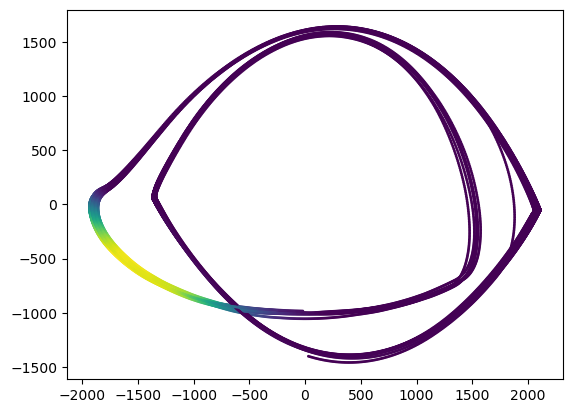
\includegraphics[width=0.45\textwidth]{images/p1.png}}
\subfigure[area 2]{
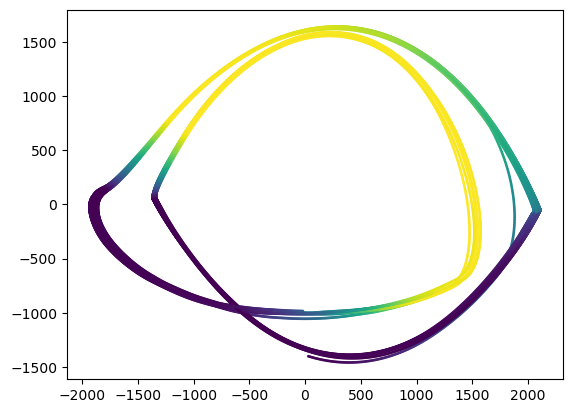
\includegraphics[width=0.45\textwidth]{images/p2.png}}
\subfigure[area 3]{
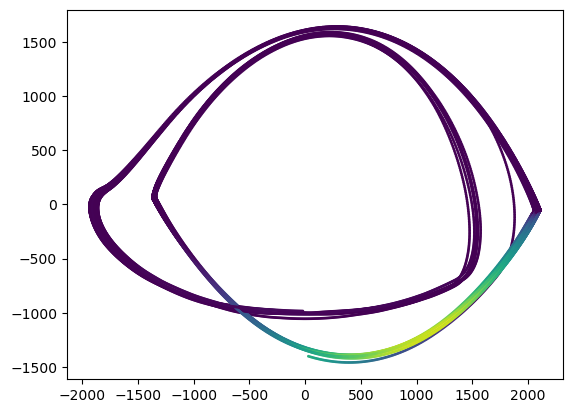
\includegraphics[width=0.45\textwidth]{images/p3.png}}
\caption{The area occupations shown on the PCA'd data part 1}
\label{fig:PCAoccs1}
\end{figure}

\begin{figure}[H]
\centering
\subfigure[area 4]{
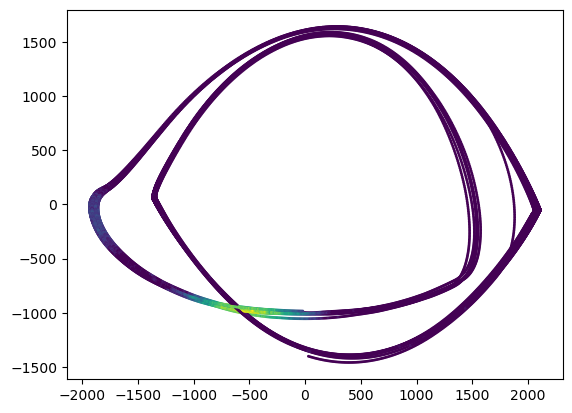
\includegraphics[width=0.45\textwidth]{images/p4.png}}
\subfigure[area 5]{
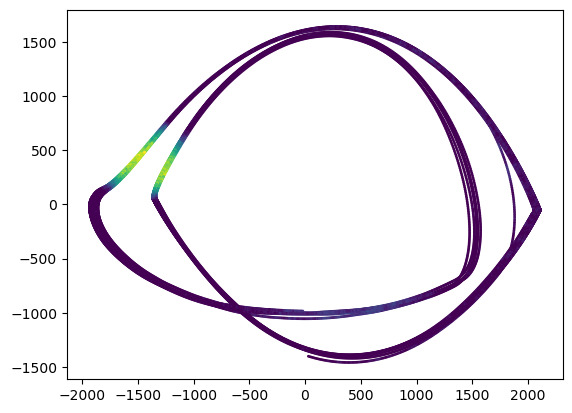
\includegraphics[width=0.45\textwidth]{images/p5.png}}
\subfigure[area 6]{
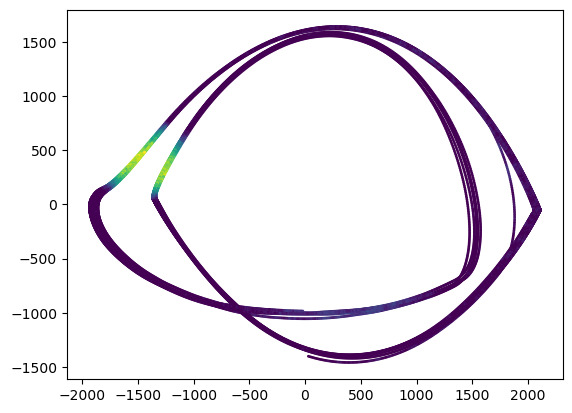
\includegraphics[width=0.45\textwidth]{images/p6.png}}
\caption{The area occupations shown on the PCA'd data part 2}
\label{fig:PCAoccs2}
\end{figure}

\begin{figure}[H]
\centering
\subfigure[area 7]{
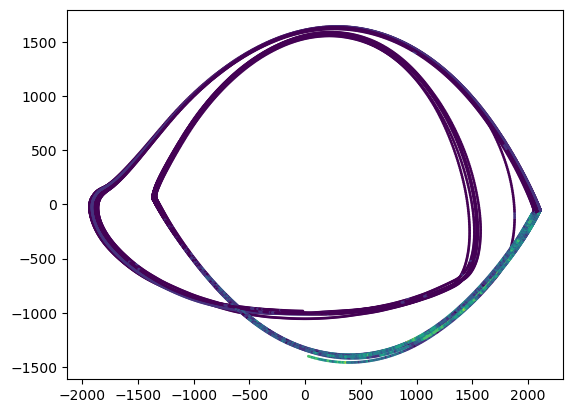
\includegraphics[width=0.45\textwidth]{images/p7.png}}
\subfigure[area 8]{
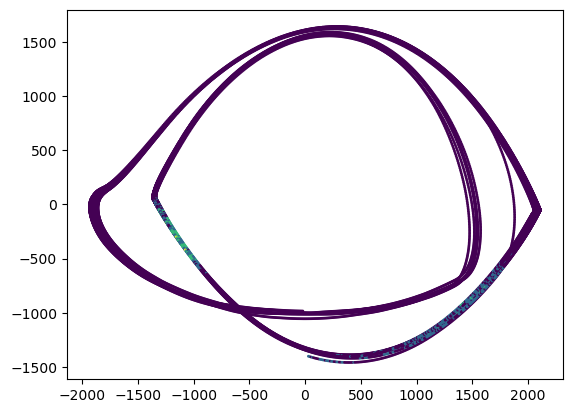
\includegraphics[width=0.45\textwidth]{images/p8.png}}
\subfigure[area 9]{
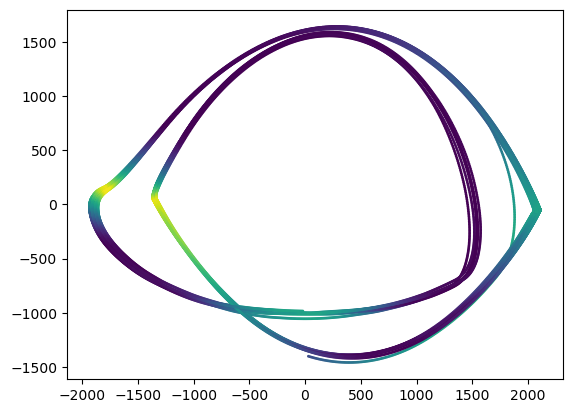
\includegraphics[width=0.45\textwidth]{images/p9.png}}
\caption{The area occupations shown on the PCA'd data part 3}
\label{fig:PCAoccs3}
\end{figure}

Calculating the arclength deltas can be done simply by calculating the distance between subsequent embeddings and dividing by the time distance between these embeddings (this is always one since the data is continuous). Calculating arclength traversed can be done by taking a cumulative sum of arclength deltas.

Most machine learning approaches require the data to lie in one specific interval. This is especially true for radial basis splines where each spline only covers a specific interval with non-negligeble values. If we are to predict into a before unknown range of time we therefore need to somehow take the data and represent it in a time independent manner.

The easiest way to do this is to learn a period $l$ of the data by sampling and trying different values. The easiest way to determine this period is to define a function $r$ that takes the first $l$ items and repeats this subsequence to create a sequence as long as the training input. Then we can take the $l2$ loss between the target sequence and sequences parametrized by $l$ and take the $l$ parameter with the lowest loss.

This immediately gives us a relatively good approximation of the dependency between the arc-length delta and the time \ref{fig:predictingarlenderivative}.

\begin{figure}[H]
\centering
\subfigure[Fitting the original function blue is the original orange is the fit]{
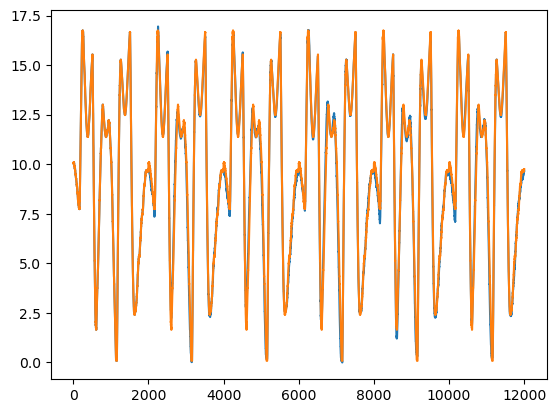
\includegraphics[width=0.45\textwidth]{images/predictingarlenderivative1.png}}
\subfigure[Predicting into the future]{
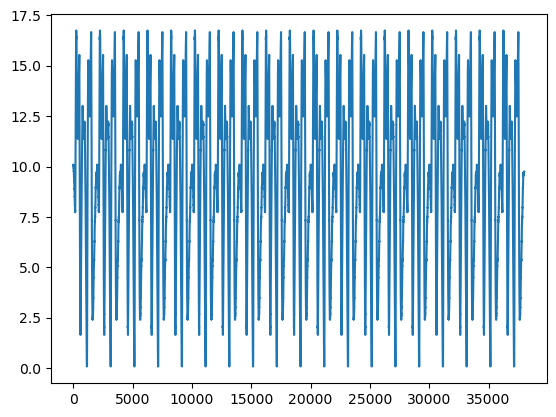
\includegraphics[width=0.45\textwidth]{images/predictingarlenderivative12.png}}
\caption{Plots of approximating the arclen derivative}
\label{fig:predictingarlenderivative}
\end{figure}

We could directly use this to learn the dependency between the arc-length delta and the first measurement area utilisation delta. This is a bad idea because in a cumulative sum even small errors accumulate over time.

The solution we chose in the end was to use the arc-length traversed as the data and the first measurement area utilisation as labels. To calculate the test data beyond the measured area we use the aforementioned time and arc-length delta dependency and cumulative sum the arc-length delta to get the arc-length traversed \ref{fig:predictingarea1}. In order to remove the before mentioned issue with the data intervals we modulo the test data with the largest input data-point.

We used the radial basis function linear regression to get the predictor. The hyper-parameters were chosen by grid-search. Values of L were from range $[2,5]$ and $\epsilon$ from $\{1+200\times x | x \in [1,24]\}$. Again the $l2$ distance between sequences was used as the loss. The search didn't seem to help too much as when the loss is multiplied by $-1$ (ie. taking the maximum loss rather than the minimal one) the result does not significantly change.


\begin{figure}[H]
\centering
\subfigure[Fitting the original function blue is the original orange is the fit]{
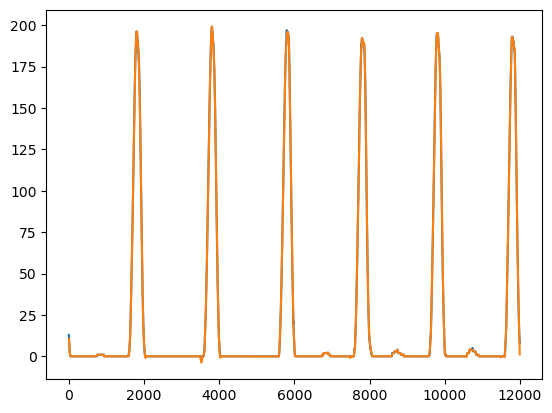
\includegraphics[width=0.45\textwidth]{images/predictingarea1.png}}
\subfigure[Predicting into the future]{
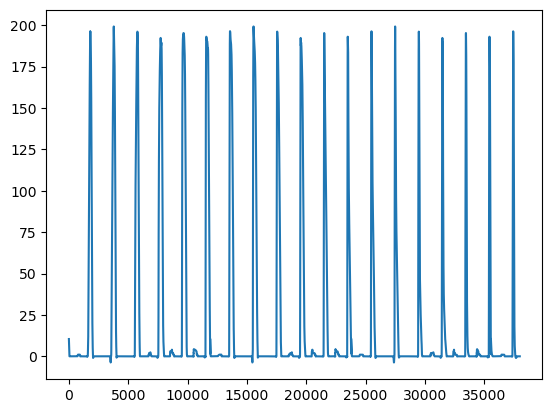
\includegraphics[width=0.45\textwidth]{images/predictingarea12.png}}
\caption{Plots of approximating area 1}
\label{fig:predictingarea1}
\end{figure}

\end{task}